\documentclass{article}
\usepackage[final]{neurips_2020}

\usepackage[utf8]{inputenc}
\usepackage{ctex}
\usepackage[T1]{fontenc}    % use 8-bit T1 fonts
\usepackage{hyperref}       % hyperlinks
\usepackage{url}            % simple URL typesetting
\usepackage{booktabs}       % professional-quality tables
\usepackage{amsfonts}       % blackboard math symbols
\usepackage{amsmath}
\usepackage{nicefrac}       % compact symbols for 1/2, etc.
\usepackage{microtype}      % microtypography
\usepackage{indentfirst}
\usepackage{listings}
\usepackage{graphicx}
\usepackage{graphics}
\usepackage{float}
\usepackage[dvipsnames]{xcolor}
\lstset{
    language=Python, % 设置语言
    basicstyle=\ttfamily, % 设置字体族
    breaklines=true, % 自动换行
    keywordstyle=\bfseries\color{NavyBlue}, % 设置关键字为粗体,颜色为 NavyBlue
    morekeywords={}, % 设置更多的关键字,用逗号分隔
    emph={self}, % 指定强调词,如果有多个,用逗号隔开
    emphstyle=\bfseries\color{Rhodamine}, % 强调词样式设置
    commentstyle=\itshape\color{black!50!white}, % 设置注释样式,斜体,浅灰色
    stringstyle=\bfseries\color{PineGreen!90!black}, % 设置字符串样式
    columns=flexible,
    numbers=left, % 显示行号在左边
    numbersep=2em, % 设置行号的具体位置
    numberstyle=\footnotesize, % 缩小行号
    frame=single, % 边框
    framesep=1em, % 设置代码与边框的距离
    showstringspaces=false
}
\setlength{\parindent}{2em}

\title{大作业:优化算法实验}

\author{%
    21307099 李英骏\\
    \texttt{liyj323@mail2.sysu.edu.cn} \\
}

\begin{document}
\maketitle
\tableofcontents

邻近算子\section{问题描述}
考虑一个10节点的分布式系统。节点$i$有线性测量$b_i = A_i \mathbf{x} + \mathbf{e}_i$,其中$b_i$为$5$维的测量值,$A_i$为$5 \times 200$维的测量矩阵,$\mathbf{x}$为$200$维的未知稀疏向量且稀疏度为$5\%$,$\mathbf{e}_i$为$5$维的测量噪声。从所有$b_i$与$A_i$中恢复$\mathbf{x}$的一范数正则化最小二乘模型如下:
\begin{equation}
    \min_{\mathbf{x}} \left( \frac{1}{2} \sum_{i=1}^{10} \|\mathbf{A}_i \mathbf{x} - \mathbf{b}_i\|_2^2 + \lambda \|\mathbf{x}\|_1 \right)
    \label{eq: original_problem}
\end{equation}
其中$\lambda > 0$为正则化参数。设计下述算法求解该问题:
\begin{enumerate}
    \item 邻近点梯度法;
    \item 交替方向乘子法;
    \item 次梯度法;
\end{enumerate}
在实验中,设$\mathbf{x}$的真值中的非零元素服从均值为$0$方差为$1$的高斯分布,$A_i$中的元素服从均值为$0$方差为$1$的高斯分布,$\mathbf{e}_i$中的元素服从均值为$0$方差为$0.1$的高斯分布。对于每种算法,请给出每步计算结果与真值的距离以及每步计算结果与最优解的距离。此外,请讨论正则化参数$\lambda$对计算结果的影响。

\setlength{\parindent}{0em}
\section{算法设计}
\subsection{邻近点梯度法}
\subsubsection{算法介绍}
\noindent\fbox{%
    \parbox{\textwidth}{\emph{邻近算子 (proximity operator):}%
        \begin{equation}
            \text{prox}_f (x) = \arg\min_{y \in \mathbb{R}^n} f(y) + \frac{1}{2} \| x - y \|_2^2,
        \end{equation}

        \emph{投影算子 (projection operator):}
        \begin{equation}
            \text{proj}_X (x) = \arg\min_{y \in X} \| y - x \|_2^2,
        \end{equation}

        \emph{软门限法 (soft thresholding):}
        \[
            \arg\min_X \|X - B\|_2 + \lambda \|X\|_1 \text{  的解为}
        \]
        \begin{equation}
            \text{soft}(B, \lambda/2) =
            \begin{cases}
                B + \lambda/2, & \text{if } B < -\lambda/2     \\
                0,             & \text{if } |B| \leq \lambda/2 \\
                B - \lambda/2, & \text{if } B > \lambda/2
            \end{cases}
        \end{equation}
        即
        \begin{equation}
            \text{soft}(B, \lambda/2) = \text{sign}(B) * \max (|B| - \lambda/2,0)
            \label{eq: softthresholding}
        \end{equation}
    }
}

若函数$f_0$有结构非光滑,则
\begin{equation}
    \min_x f_0(x) = s(x) + r(x)
\end{equation}
其中$s(x)$是光滑部分,$r(x)$是非光滑部分。\\
则对光滑的$s(x)$部分可以做梯度下降:
\begin{equation}
    x^{k+\frac{1}{2}} = x^k - \alpha \cdot \nabla s (x^k)
    \label{eq: eq1.1}
\end{equation}
对非光滑的$r(x)$做邻近点投影
\begin{equation}
    \min_{x} r(x) + \frac{1}{2\alpha} \|\ x - \hat{x}\ \|,
\end{equation}
从而得到递推方程
\begin{equation}
    x^{k+1} = \arg\min_{x} r(x) + \frac{1}{2\alpha} \| x - x^{k+\frac{1}{2}} \|_2^2
    \label{eq: eq1.2}
\end{equation}
\newpage
\subsubsection{具体算法说明}
将原问题(\ref{eq: original_problem})代入上述式(\ref{eq: eq1.1})(\ref{eq: eq1.2}),
可得:
\begin{equation}
    s(x) = \frac {1}{2} \sum_{i=1}^{10} \|\mathbf{A}_i \mathbf{x} - \mathbf{b}_i\|_2^2
\end{equation}
\begin{equation}
    r(x) =  \lambda \|\mathbf{x}\|_1
\end{equation}
则式(\ref{eq: eq1.1})特化为:
\begin{equation}
    x^{k+\frac{1}{2}} = x^k - \alpha * \sum_{i=1}^{10} \mathbf{A_i^T} (\mathbf{A}_i x^k - \mathbf{b}_i)
    \label{eq: eq1.3}
\end{equation}
式(\ref{eq: eq1.2})特化为:
\begin{equation}
    x^{k+1} = \arg\min_x (\lambda\|x\|_1 + \frac{1}{2 \alpha} \|x - x^{k+\frac{1}{2}}\|_2^2)
    \label{eq: eq1.4}
\end{equation}
其软门限法优化步为
\begin{equation}
    x^{k+1} = \text{sign}(x^{x+\frac{1}{2}}) * \max (|x^{x+\frac{1}{2}}| - \alpha*\lambda,0)
    \label{eq: eq1.5}
\end{equation}

\subsubsection{代码实现}
\begin{lstlisting}
    class ProximalGradientDescent:
        def __init__(self, alpha, lambda_val, stop=1e-5, max_iter=100000):
            self.alpha = alpha
            self.lambda_val = lambda_val
            self.stop = stop
            self.max_iter = max_iter

        def gradient_step(self, A, b, x_k):
            gradient = np.sum([A_i.T @ ((A_i @ x_k) - b_i)
                            for A_i, b_i in zip(A, b)], axis=0)
            return x_k - self.alpha * gradient

        def soft_thresholding_1(self, x_k_half):
            for i in range(len(x_k_half)):
                if x_k_half[i] < - self.lambda_val*self.alpha:
                    x_k_half[i] = x_k_half[i] + self.lambda_val*self.alpha
                elif x_k_half[i] > self.lambda_val*self.alpha:
                    x_k_half[i] = x_k_half[i] 
                    - self.lambda_val*self.alpha
\end{lstlisting}
\newpage
\begin{lstlisting}[firstnumber=20]
                else:
                    x_k_half[i] = 0.0
                return x_k_half

        def check_convergence(self, x_k, x_k_ud):
            return np.linalg.norm((x_k_ud - x_k), 2) < self.stop

        def fit(self, A, b, x_true):
            Xk = np.zeros_like(x_true)
            X_opt_step = np.zeros(
            (self.max_iter, x_true.shape[0], x_true.shape[1]))
            count = 0
            while count < self.max_iter:
                Xk_half = self.gradient_step(A, b, Xk)
                Xk_ud = self.soft_thresholding_1(Xk_half)
                #print(Xk_ud.shape)
                print("Iter ", count+1, ":", np.linalg.norm((Xk_ud - x_true), 2))

                X_opt_step[count] = Xk_ud
                if self.check_convergence(Xk, Xk_ud):
                    print("DONE")
                    break

                Xk = Xk_ud
                count += 1

            return X_opt_step[:count + 1,:]
\end{lstlisting}
\noindent
代码的8-11行, gradient\_step函数计算了式(\ref{eq: eq1.3}), 13-20行计算了式(\ref{eq: eq1.4}),\\
24-25行的函数用于检验终止条件,即两次迭代的结果的2-norm距离小于$10^{-5}$。\\
fit函数为主要迭代部分。\\
将软门限法的实现向量化如下(即式(\ref{eq: eq1.5})),经实验可提升40\%左右的性能。
\begin{lstlisting}
    def soft_thresholding_1(self, x_k_half):
        x_k_half = np.sign(x_k_half) * np.maximum((np.abs(x_k_half)-self.alpha*self.lambda_val),0)
        return x_k_half
\end{lstlisting}
\subsection{交替方向乘子法}
\subsubsection{算法介绍}
对于优化问题
\begin{align}
    \min f_1(x)+f_2(x) \\
    s.t. Ax+By = 0
\end{align}
则其优化步为:
\begin{align}
     & x^{k+1} = \arg\min_x \text{L}_\rho\left(x, y^k,\lambda^k\right)              \\
     & y^{k+1} = \arg\min_y \text{L}_\rho\left(x^{k+1}, y,\lambda^k\right)          \\
     & \lambda^{k+1} = \lambda^k + \rho\left(\text{A}x^{k+1}+\text{B}y^{k+1}\right)
\end{align}

\subsubsection{具体算法说明}
将原问题将原问题(\ref{eq: original_problem})代入(即加入约束$x-y=0$),有
\begin{align}
     & f_1(x) = \frac {1}{2} \sum_{i=1}^{10} \|\mathbf{A}_i \mathbf{x} - \mathbf{b}_i\|_2^2 \\
     & f_2(y) = \lambda \|y\|_1
\end{align}
其增广拉氏函数为:
\begin{equation}
    L_c(x,y,t) = \frac {1}{2} \sum_{i=1}^{10} \|\mathbf{A}_i \mathbf{x} - \mathbf{b}_i\|_2^2+
    \lambda\|y\|_1+<t, x-y>+\frac{\rho}{2}\|x-y\|_2^2
    \label{eq: lc}
\end{equation}

得迭代方程(\emph{此处用t代表上面的$\lambda$,防止写码的时候和原问题的正则项权重$\lambda$搞混淆}):
\begin{align}
    x^{k+1} & = \left(\sum_{i=1}^{10} A_i^T A_i+\rho I\right)^{-1}\left(\sum_{i=1}^{10}A_i^T b +\rho y^k -t^k\right) \label{eq: 2.1} \\
    y^{k+1} & = \arg\min_y \lambda \|y\|_1 + \frac{\rho}{2}\|y-x^{k+1}-\frac{t^k}{\rho}\|_2^2 \label{eq: 2.2}                        \\
    t^{k+1} & = t^{k} + \rho(x^{k+1}-y^{k+1}) \label{eq: 2.3}
\end{align}
其中x项部分是光滑的,直接求偏导即得,y项部分需用软门限法(\ref{eq: softthresholding}),优化步如下:
\begin{align}
    y^{k+1} & = \mathbf{sign} (x^{k+1}+\frac{t^{k}}{\rho}) * \max (|x^{k+1}+\frac{t^{k}}{\rho}| - \frac{1}{2}\cdot\frac{2}{c}\lambda)   \\
            & = \mathbf{sign} (x^{k+1}+\frac{t^{k}}{\rho}) * \max (|x^{k+1}+\frac{t^{k}}{\rho}| - \frac{\lambda}{\rho}) \label{eq: 2.4}
\end{align}
\newpage
\subsubsection{代码实现}
\begin{lstlisting}
    class ADMM:
        def __init__(self, rho, lamda, x_dim, b_dim, stop=1e-5, max_iter=100000):
            self.rho = rho
            self.lamda = lamda
            self.stop = stop
            self.max_iter = max_iter
            self.x_dim = x_dim
            self.b_dim = b_dim

        def update_x(self, A, b, Y, T):
            A_T = self.rho * np.eye(self.x_dim)
            A_b = np.zeros((self.x_dim, 1))

            for i in range(10):
                A_T += A[i].T @ A[i]
                A_b += A[i].T @ b[i]

            A_T_inv = np.linalg.inv(A_T)
            X_update = A_T_inv @ (A_b + self.rho * Y - T)
            return X_update

        def update_y(self, X, T):
            Y_update = np.sign(X + T / self.rho) * np.maximum(np.abs(X +
            T / self.rho) - self.lamda / self.rho, 0)
            return Y_update

        def update_t(self, T, X, Y):
            T_update = T + self.rho * (X - Y)
            return T_update

        def check_convergence(self, x_k, x_k_ud):
            return np.linalg.norm((x_k_ud - x_k), 2) < self.stop
\end{lstlisting}
\newpage
\begin{lstlisting}[firstnumber=33]
        def fit(self, A, b, x_true):
            # 初始化 X, Y, T
            X = np.zeros((self.x_dim, 1))
            Y = np.zeros((self.x_dim, 1))
            T = np.zeros((self.x_dim, 1))
            count = 0
            X_opt_step = np.zeros(
                (self.max_iter, x_true.shape[0], x_true.shape[1]))

            while count < self.max_iter:
                X_update = self.update_x(A, b, Y, T)
                Y_update = self.update_y(X_update, T)
                T_update = self.update_t(T, X_update, Y_update)

                X_opt_step[count] = X_update
                print("Iter ", count+1, ":", np.linalg.norm((X_update - x_true), 2))
                if self.check_convergence(X_update, X):
                    break

                # 更新 X, Y, T
                X, Y, T = X_update, Y_update, T_update
                count += 1
            return X_opt_step[:count + 1, :]
\end{lstlisting}
10-20行的update\_x函数实现了式(\ref{eq: 2.1}), 22-25行的update\_y实现了式(\ref{eq: 2.4}),
27-29行的update\_t实现了式(\ref{eq: 2.3}),fit函数为主要迭代部分,按顺序依次调用三个函数并记录每步优化结果。

\newpage
\subsection{次梯度法}
\subsubsection{算法介绍}
\begin{equation}
    x^{k+1} = x^k - \alpha^k * g_0(x^k), g_0 \in \partial f_0(x)
\end{equation}

\subsubsection{具体算法说明}
对于原问题(\ref{eq: original_problem}),$g_0$有以下三种情形:
\begin{equation}
    g_0(x) =
    \begin{cases}
        \sum_{i=1}^{10}A_i^T(A_i x-b) + \lambda,                                & \text{if } x>0 \\
        \sum_{i=1}^{10}A_i^T(A_i x-b) + \lambda * \text{rand}\left[-1,1\right], & \text{if } x=0 \\
        \sum_{i=1}^{10}A_i^T(A_i x-b) - \lambda,                                & \text{if } x<0
    \end{cases}
    \label{eq: eq3.1}
\end{equation}
我选择$\alpha$为变长步长
\begin{equation}
    \alpha^{k+1} = \frac{\alpha^k}{\sqrt{step+1}}
    \label{eq: eq3.2}
\end{equation}

\subsubsection{代码实现}
\begin{lstlisting}
    class SubgradientMethod:
        def __init__(self, lamda, alpha, x_dim, b_dim, stop=1e-5, max_iter=80000):
            self.lamda = lamda
            self.alpha = alpha
            self.stop = stop
            self.max_iter = max_iter
            self.x_dim = x_dim
            self.b_dim = b_dim

        def check_convergence(self, x_k, x_k_ud):
            return np.linalg.norm((x_k_ud - x_k), 2) < self.stop
\end{lstlisting}
上方函数主要用于初始化和检测终止条件。
\newpage
\begin{lstlisting}[firstnumber=12]
        def fit(self, A, b, x_true):
            X_temp = np.zeros((self.x_dim, 1))
            count = 0
            X_opt_step = np.zeros(
                (self.max_iter, x_true.shape[0], x_true.shape[1]))

            while count < self.max_iter:
                g = np.zeros((self.x_dim, 1))
                for i in range(len(A)):  # 遍历A中的每个矩阵A_i
                    g += A[i].T @ (A[i] @ X_temp - b[i].reshape(-1, 1))

                X_new = np.array([np.random.uniform(-1, 1) if x ==
                                0 else np.sign(x) for x in X_temp]).reshape(-1, 1)
                g += self.lamda * X_new
                alphak = self.alpha / np.sqrt(count + 1)
                X_update = X_temp - alphak * g
                print("Iter ", count+1, ":", np.linalg.norm((X_update - x_true), 2))
                X_opt_step[count] = X_update
                if self.check_convergence(X_update, X_temp):
                    break

                X_temp = X_update
                count += 1

            return X_opt_step[:count + 1, :]
\end{lstlisting}
fit函数的20-27行实现了式(\ref{eq: eq3.1})的功能,其中26行实现了式(\ref{eq: eq3.2})的功能。 \newpage
\section{其他代码实现}
\subsection{数据生成}
\begin{lstlisting}
    def generate_data(x_dim, b_dim, sparsity, seed=42):
        np.random.seed(seed)

        x_true = np.zeros((x_dim,1))
        non_zero_indices = np.random.choice(
            x_dim, int(sparsity * x_dim), replace=False)
        x_true[non_zero_indices,0] = np.random.randn(int(sparsity * x_dim))
        # generate A_i
        A = [np.random.randn(b_dim, x_dim) for _ in range(10)]

        # generate noise e_i
        e = [np.random.randn(b_dim,1) * np.sqrt(0.1) for _ in range(10)]

        # generate b_i
        b = [A_i @ x_true + e_i for A_i, e_i in zip(A, e)]

        return x_true, A, e, b
\end{lstlisting}
我锁定了seed以保证可重复性,并且在data\_generator.py中验证了均值和方差满足条件。如下图
\begin{figure}[H]
    \centering
    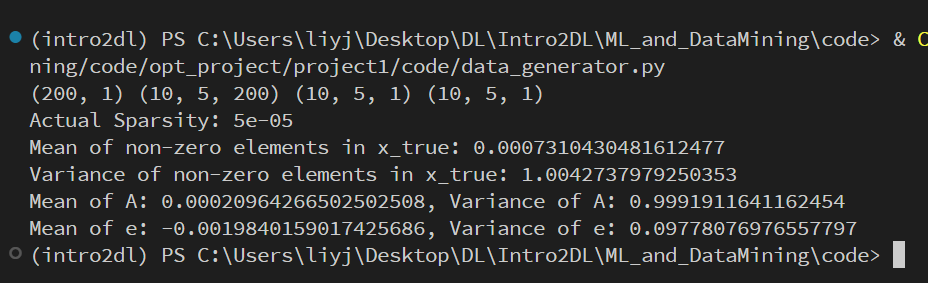
\includegraphics[width=\linewidth]{./images/Figure_test_0.png}
    \caption{数据生成器测试}
\end{figure}
\newpage
\section{数值实验及结果分析}
\subsection{邻近点梯度法}
取$\alpha=0.001$
\begin{figure}[H]
    \centering
    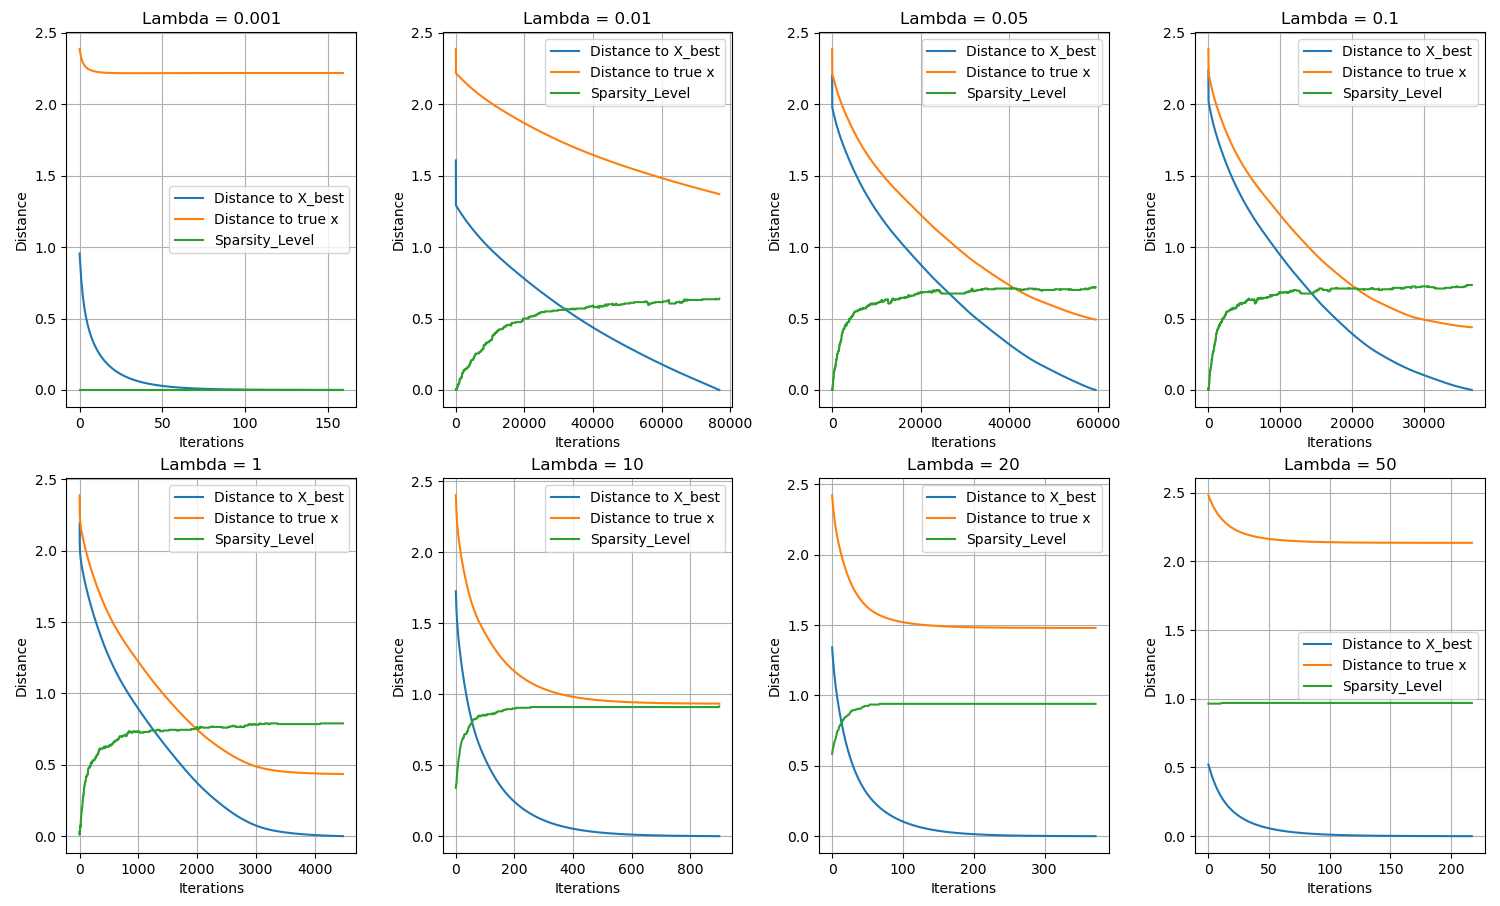
\includegraphics[width=\linewidth]{./images/Figure_1.png}
    \caption{邻近点梯度法}
\end{figure}
观察蓝色曲线(与最优解的2-norm距离,可以认为反映了收敛速度)可以看出,随着$\lambda$增大,函数的收敛速度加快。这可能是因为稀疏化正则项的优化速度更快,当它权重更大时自然收敛得更快。\\
同时观察橙色曲线(与真实值的距离)可以发现,在合适的$\lambda$范围内(大约在0.1-1),函数可以被优化到最接近真实的X,此时可以认为最小二乘项的权重和稀疏正则化项的权重比例是合适的\\
另外,观察绿色曲线可以很自然地发现,当$\lambda$较小(0.001)时,结果几乎是稠密的;而随着$\lambda$增大,结果越来越稀疏;$\lambda>10$后,结果几乎是完全稀疏的。且稀疏程度随着迭代次数提高。
\newpage
\subsection{交叉方向乘子法}
我们选定$\rho=0.005$,观察如下式(\ref{eq: lc})可以发现:
\begin{equation*}
    L_c(x,y,t) = \frac {1}{2} \sum_{i=1}^{10} \|\mathbf{A}_i \mathbf{x} - \mathbf{b}_i\|_2^2+
    \lambda\|y\|_1+<t, x-y>+\frac{\rho}{2}\|x-y\|_2^2
\end{equation*}
当$\lambda$较大时,函数更好地约束了$y$的稀疏度,但响应地$\|x-y\|_2^2$的权重减少,即减弱了对条件$x - y =0$的约束,反而会降低$x$的稀疏程度。
实验如下:\\
\subsubsection{当$\lambda$相比$\rho$较大时}
\paragraph{以向量中零元素的数量计算稀疏度(标准算法)\\}
实验结果见下图(\ref{fig: img2.0})。\\
\begin{enumerate}
    \item 观察橙、蓝曲线可以看出,随着$\lambda$增加,算法收敛得更慢,在过大时甚至不收敛。
    \item 观察橙色曲线,可以发现在$lambda\leq1$时,算法都可以收敛到一个较为接近$x\_true$的结果上,但更大的$\lambda$会导致最小二乘项的权重下降,从而使迭代振荡得更加剧烈。
    \item 观察绿色曲线,可以发现当以零元素的数量计算稀疏度时,矩阵几乎是不稀疏的(稀疏度$\approx0$),这是因为稀疏化正则项和软门限(这是直接产生严格0的主要渠道)都作用在y上,通过$\|x-y\|_2^2$很难产生出严格的0值。
\end{enumerate}

\begin{figure}[H]
    \centering
    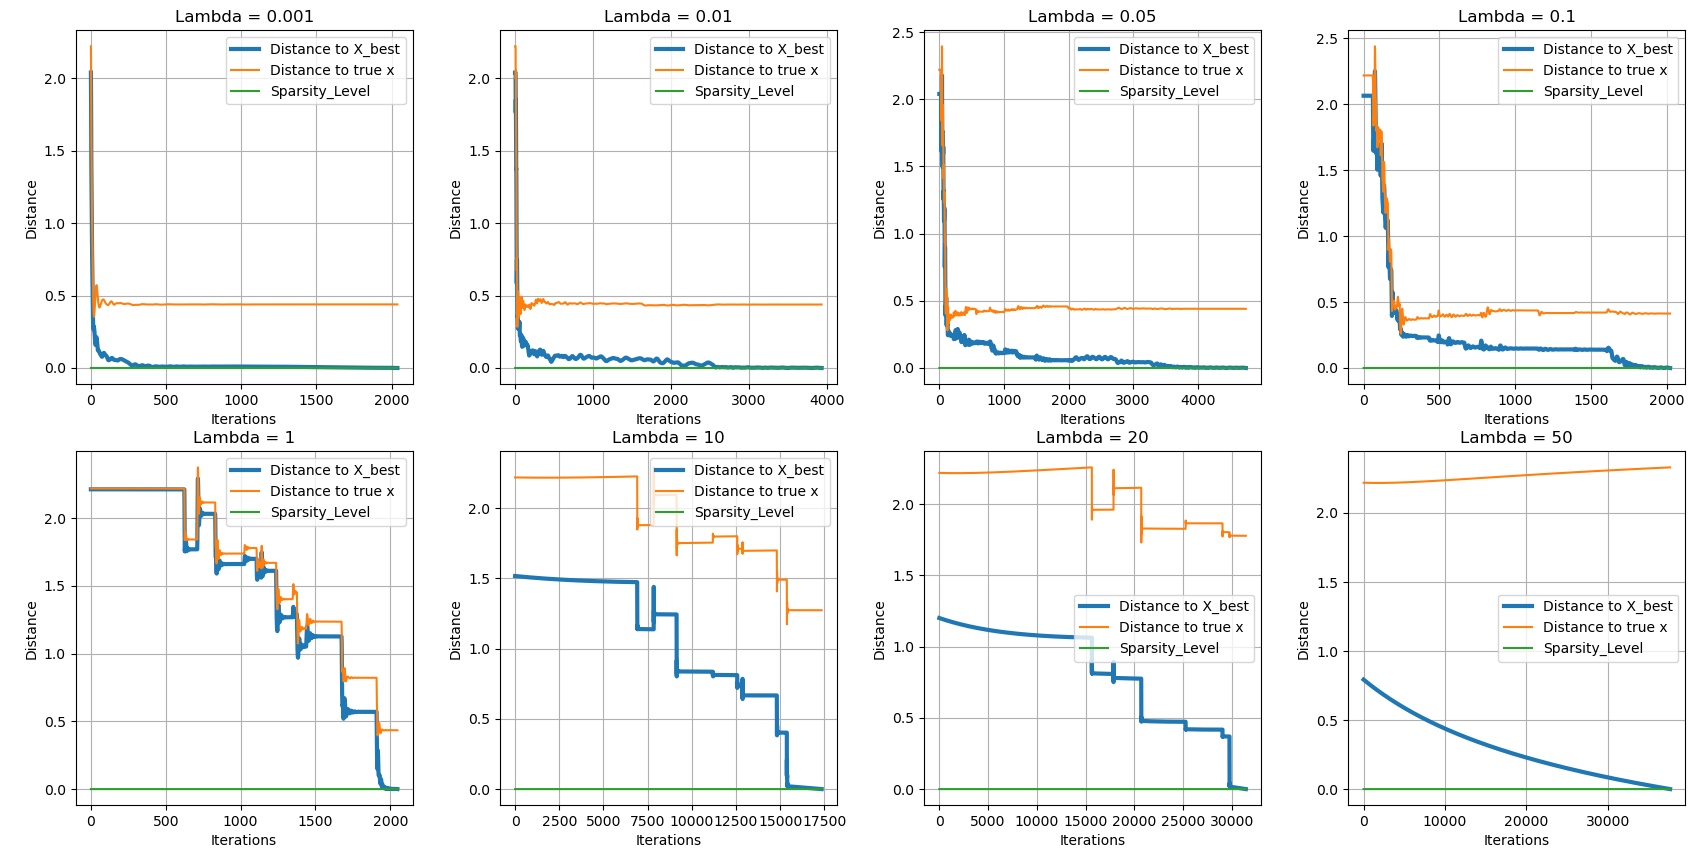
\includegraphics[width=\linewidth]{./images/Figure_2.png}
    \caption{交叉方向乘子法 2.0}
    \label{fig: img2.0}
\end{figure}
\newpage
\paragraph{以向量中$\leq 10^{-3}$项的数量计算稀疏度(非标准算法)\\}
实验结果见下图(\ref{fig: img2.1}),可以看出这个度量较好地体现了矩阵的稀疏程度,尽管不是严格的稀疏度。
它验证了上述说法:即在$\lambda$和$\rho$的比例合适时,我们可以获得较好的稀疏度,$\lambda$过大时,稀疏度会明显下降。
\begin{figure}[H]
    \centering
    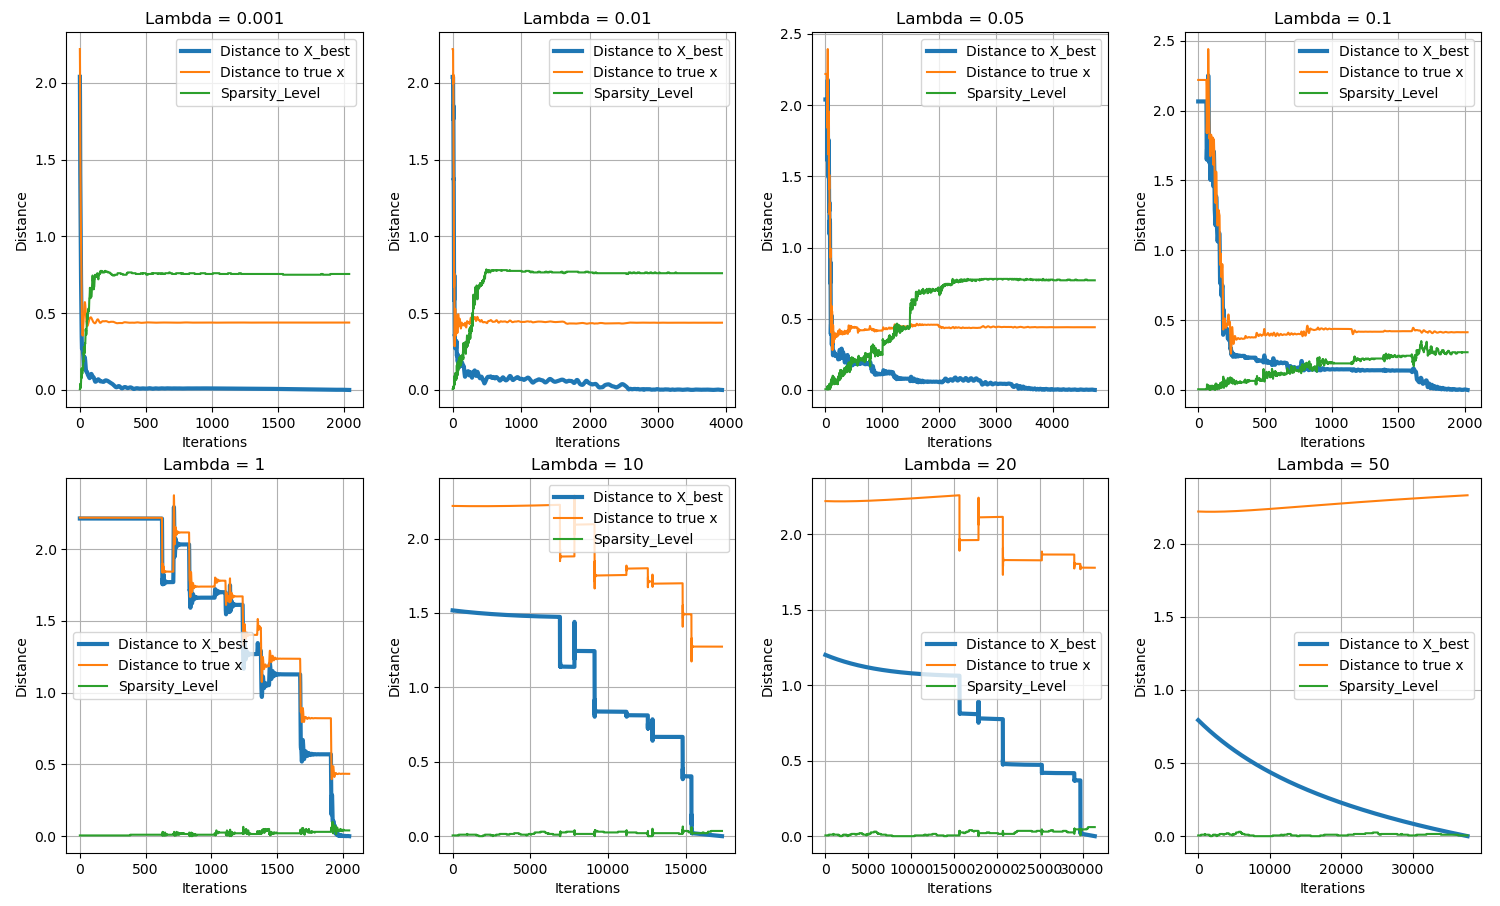
\includegraphics[width=\linewidth]{./images/Figure_2_1.png}
    \caption{交叉方向乘子法 2.1}
    \label{fig: img2.1}
\end{figure}

\subsubsection{当$\lambda$相比$\rho$较小时}
\paragraph{以向量中零元素的数量计算稀疏度(标准算法)\\}
实验结果见下图(\ref{fig: img2.2})。\\
\begin{enumerate}
    \item 观察橙、蓝曲线可以看出,随着$\lambda$增加,算法收敛得更快了。
    \item 观察橙色曲线,可以发现$lambda$取这些值时,算法都可以收敛到一个较为接近$x\_true$的结果上,但更大的$\lambda$会导致最小二乘项的权重下降,从而使迭代振荡得更加剧烈。
    \item 观察绿色曲线,可以发现当以零元素的数量计算稀疏度时,矩阵几乎是不稀疏的(稀疏度$\approx0$),这是因为稀疏化正则项和软门限(这是直接产生严格0的主要渠道)都作用在y上,通过$\|x-y\|_2^2$很难产生出严格的0值。
\end{enumerate}
\newpage

\begin{figure}[H]
    \centering
    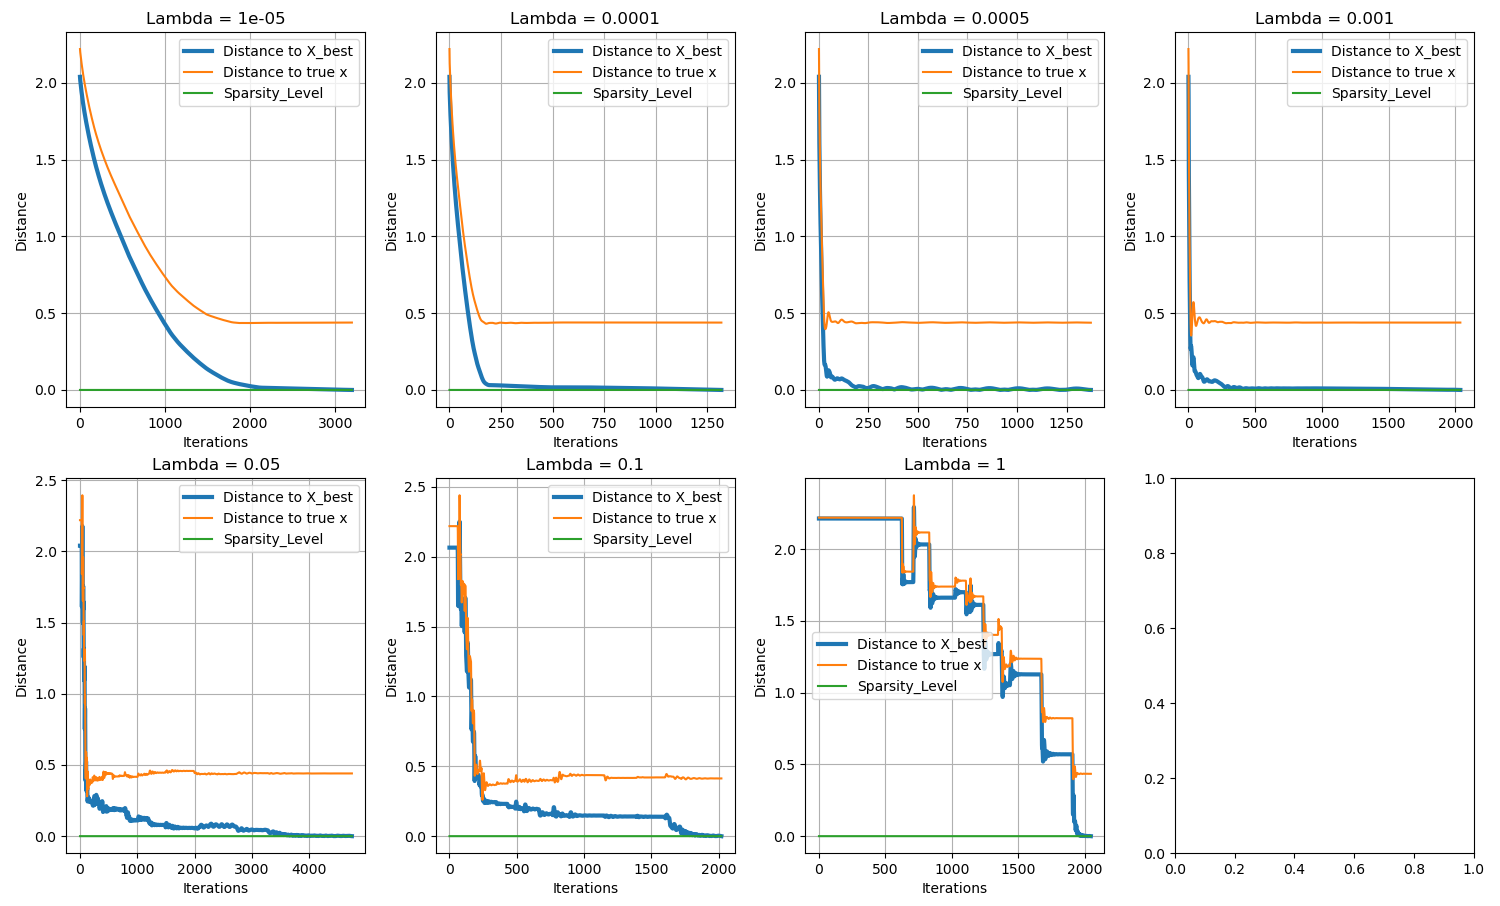
\includegraphics[width=0.9\linewidth]{./images/Figure_2_2.png}
    \caption{交叉方向乘子法 2.2}
    \label{fig: img2.2}
\end{figure}

\paragraph{以向量中$\leq 10^{-2}$,$\leq 10^{-3}$,$\leq 10^{-4}$项的数量计算稀疏度(非标准算法)\\}
实验结果见下图(\ref{fig: img2.3})。图中三条稀疏度曲线分别是Sparsity\_Level\_0:$\leq 10^{-2}$,
Sparsity\_Level\_1:$\leq 10^{-3}$,Sparsity\_Level\_2:$\leq 10^{-4}$.\\
可以看出,在$lambda\leq 0.001$时,优化结果和它的稀疏程度都较好,而当$\lambda\geq 0.05$即$\rho$时,$\leq 10^{-4}$的项的数量显著下降。
\begin{figure}[H]
    \centering
    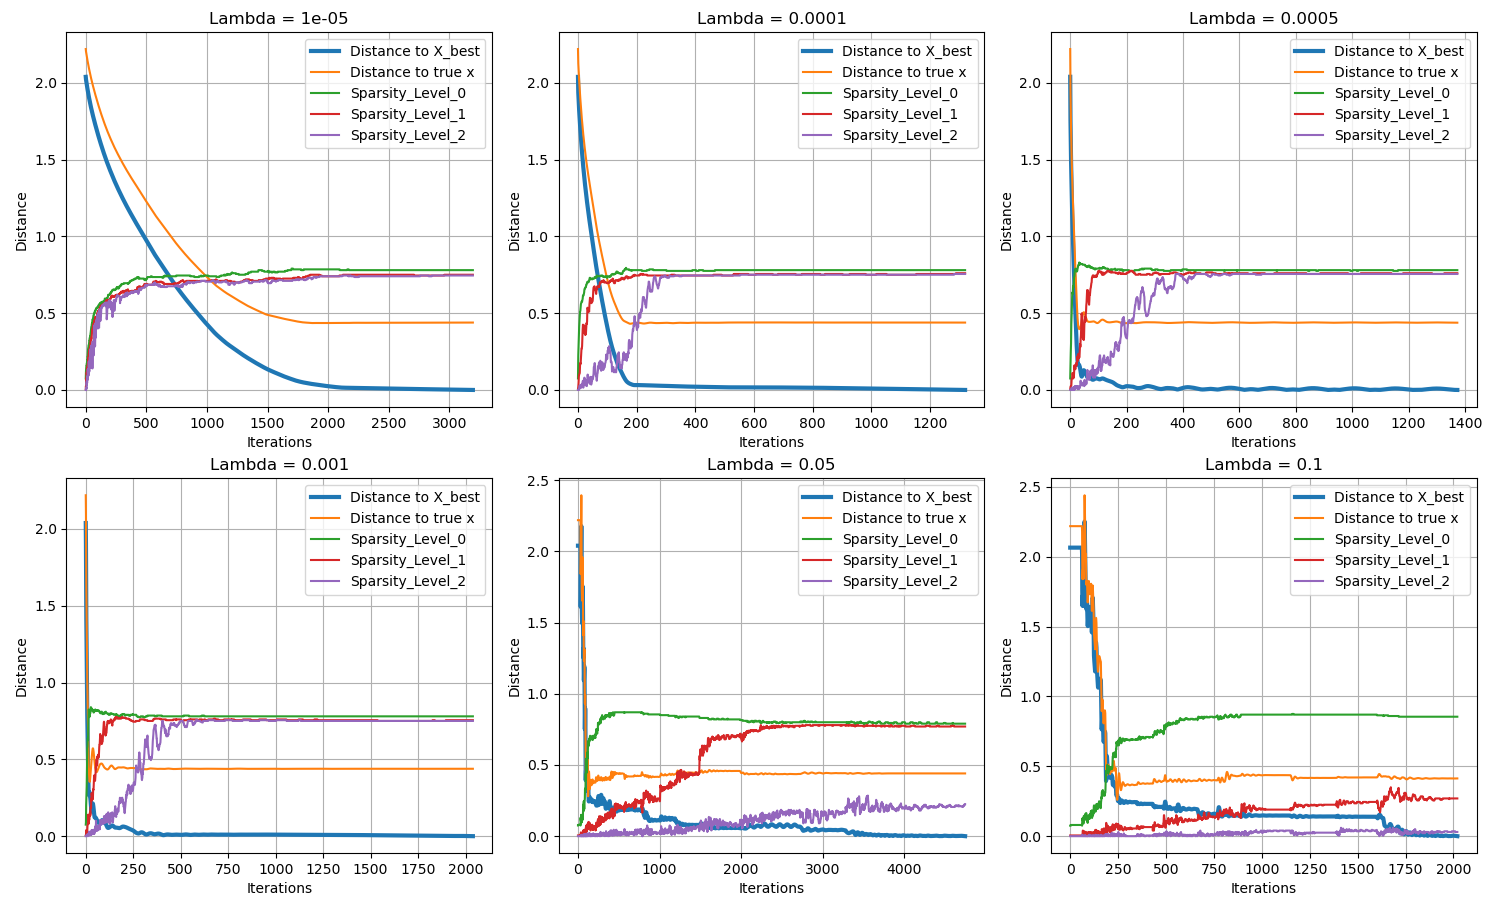
\includegraphics[width=0.9\linewidth]{./images/Figure_2_3.png}
    \caption{交叉方向乘子法 2.3}
    \label{fig: img2.3}
\end{figure}

\newpage
\subsection{次梯度法}
\subsubsection{取$\alpha=0.0001$}
实验结果如图:
\begin{figure}[H]
    \centering
    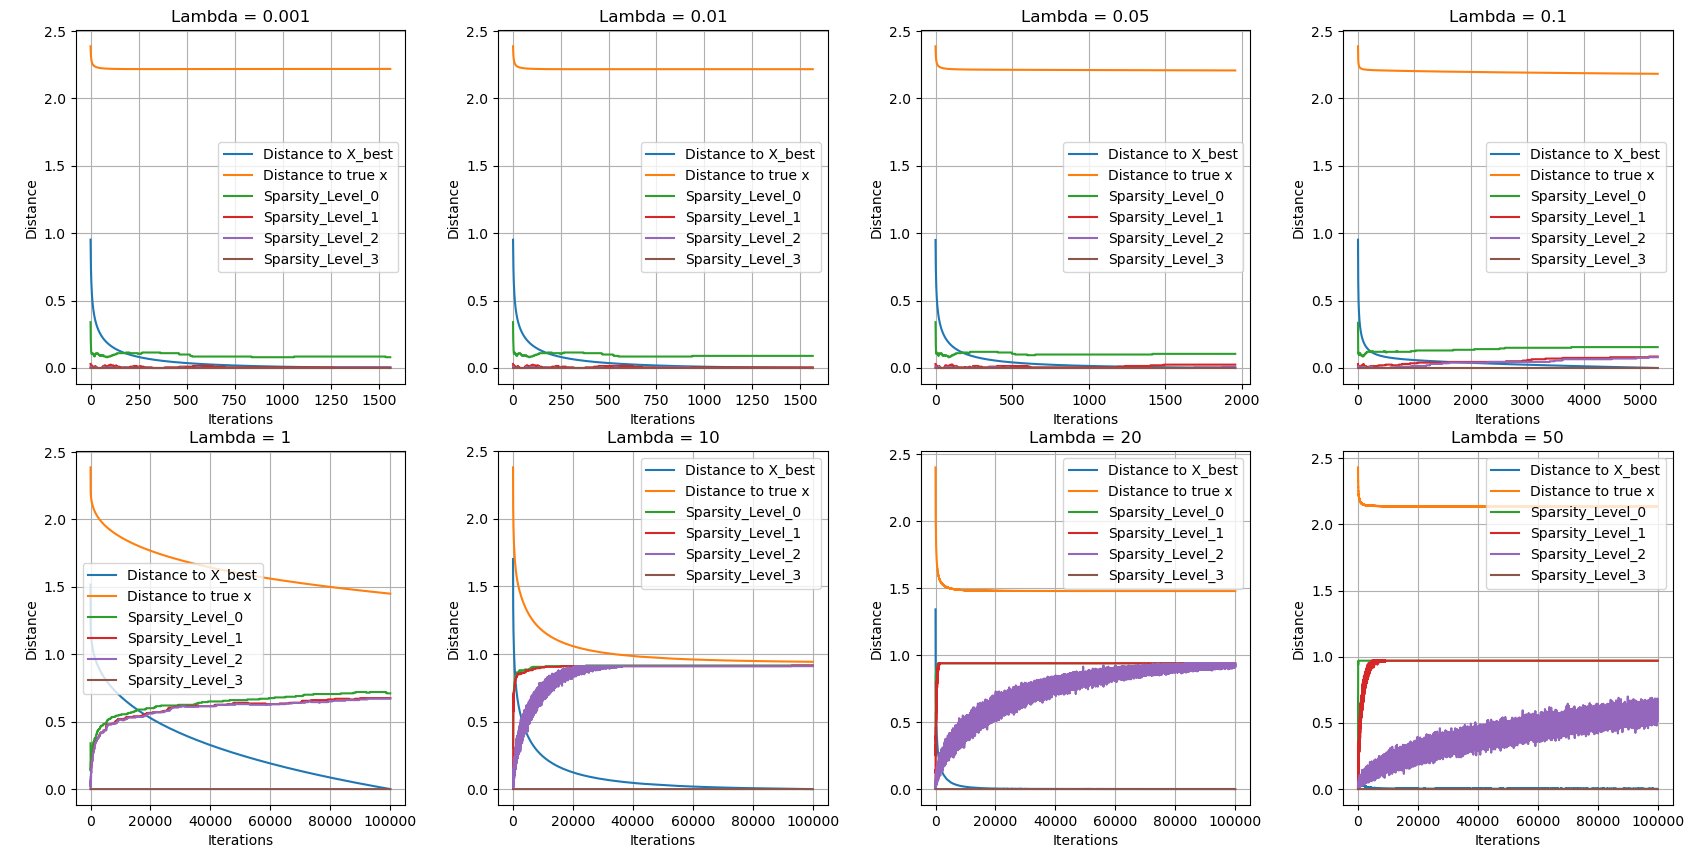
\includegraphics[width=0.9\linewidth]{./images/Figure_3_1.png}
    \caption{次梯度法}
    \label{fig: img3}
\end{figure}
图中三条稀疏度曲线分别是Sparsity\_Level\_0:$\leq 10^{-2}$,
Sparsity\_Level\_1:$\leq 10^{-3}$,Sparsity\_Level\_2:$\leq 10^{-4}$,Sparsity\_Level\_3:$=0$,
观察蓝色曲线可以发现,随着$\lambda$的增加,算法收敛先变慢后变快,在$\lambda$为1时最慢。
观察橙色曲线,可以发现,在$\lambda$取1-10左右时,函数可以收敛到最接近X\_true\\
观察剩余四色曲线,可以发现,$\lambda$取1-20时,所得值的稀疏程度较高,且均集中在$0 \sim 10^{-4}$。注意到次梯度法中,严格等于0的元素也是几乎不存在的(棕色的level3曲线一直几乎为0)。\\
另外可以注意到,即使X与X\_true和X\_best的距离已经几乎不变,$\leq10^{-4}$的项的数量仍然在一直增加,这表明算法正在一个以X\_true范数球面附近搜索。

\end{document}
